%%%%%%%%%%%%%%%%%%%%%%%%%%%%%%%%%%%%%%%%%%%%%%%%%%%%%%%%%%%%%%%%%%%%%%%%%%%%%%%%
%%%%%%%%%%%%%%%%%%%%%%%%%%%%%%%%%%%%%%%%%%%%%%%%%%%%%%%%%%%%%%%%%%%%%%%%%%%%%%%%
%%%%%%%%%%%%%%%%%%%%%%%%%%%%%%%%%%%%%%%%%%%%%%%%%%%%%%%%%%%%%%%%%%%%%%%%%%%%%%%%

\documentclass[a0,portrait]{a0poster}

% control margins here
\usepackage{geometry}
 \geometry{
 a0paper,
 left = 5cm,
 top = 4.5cm,
 right = 5cm,
 bottom = 2cm     %4.5cm
 }
\addtolength{\textwidth}{4.5cm} % width of text can be adjusted if margins above are adjusted

\usepackage{multicol} % This is so we can have multiple columns of text side-by-side
\columnsep=3em % This is the amount of white space between the columns in the poster
\columnseprule=0pt % This is the thickness of the black line between the columns in the poster

% UZH colours %%%%%%%%%%%%%%%%%%%%%%%%%%%%%%%%%%%%%%%%%%%%%%%%%%%%%%%%%%%%%%%%%%
%%%%%%%%%%%%%%%%%%%%%%%%%%%%%%%%%%%%%%%%%%%%%%%%%%%%%%%%%%%%%%%%%%%%%%%%%%%%%%%%
\usepackage[svgnames]{xcolor}
\definecolor{uzhblau100}{RGB}{0, 40, 165}
\definecolor{uzhblau80}{RGB}{51,83,183}
\definecolor{uzhockerrot100}{RGB}{220, 96, 39}
\definecolor{uzhockerrot80}{RGB}{227, 128, 82}
\definecolor{uzhflaschengruen100}{RGB}{42, 127, 98}
\definecolor{uzhflaschengruen80}{RGB}{86, 157, 133}
\definecolor{conclusion}{RGB}{204,212,237} % the conclusion box colour

% Packages %%%%%%%%%%%%%%%%%%%%%%%%%%%%%%%%%%%%%%%%%%%%%%%%%%%%%%%%%%%%%%%%%%%%%
%%%%%%%%%%%%%%%%%%%%%%%%%%%%%%%%%%%%%%%%%%%%%%%%%%%%%%%%%%%%%%%%%%%%%%%%%%%%%%%%

\usepackage{ifthen} % needed to stop horizontal line above 'Conclusions' section
\usepackage{graphicx} % Required for including images
\usepackage{mwe,tikz}\usepackage[percent]{overpic} % overlay your photo over the background
\usepackage{booktabs} % Top and bottom rules for table
\usepackage[font=small,labelfont=bf]{caption} % Required for specifying captions to tables and figures
\usepackage{amsfonts, amsmath, amsthm, amssymb} % For math fonts, symbols and environments
\usepackage{wrapfig} % Allows wrapping text around tables and figures

\usepackage{fontspec} % custom fonts
\defaultfontfeatures[Palatino]
{
    Extension = .ttf,
    UprightFont = font/LT_41167,
    BoldFont = font/LT_41169,
    ItalicFont  = font/LT_41168,
    BoldItalicFont = font/LT_41170,
}
\defaultfontfeatures[TheSans]
{
    Extension = .otf,
    UprightFont = font/TheSans-LP5Plain,
    BoldFont = font/TheSans-LP7Bld,
    ItalicFont  = font/TheSans-LP5PlainIT,
    BoldItalicFont = font/TheSans-LP7BldIT,
}
\setmainfont{TheSans} % choose your font here
\usepackage[onehalfspacing]{setspace} % remove for single spacing
\usepackage{tcolorbox} % for the conclusions box
\usepackage{blindtext} % you can remove this once you add your content
\usepackage[export]{adjustbox} % allow floating a graphic right
\usepackage{titlesec} % customising section titles
\usepackage{needspace} % prevent break between line and section title
\usepackage{nameref} % package and command to get the name of the current section (for ifthen)
\usepackage{hyperref} % Hyperlinks
\usepackage{pifont} % More styles for bullets
\usepackage{float}    % Required for the [H] option in the figure environment

\usepackage{booktabs}  
\usepackage{array} 

% Start of the poster %%%%%%%%%%%%%%%%%%%%%%%%%%%%%%%%%%%%%%%%%%%%%%%%%%%%%%%%%%
%%%%%%%%%%%%%%%%%%%%%%%%%%%%%%%%%%%%%%%%%%%%%%%%%%%%%%%%%%%%%%%%%%%%%%%%%%%%%%%%
%%%%%%%%%%%%%%%%%%%%%%%%%%%%%%%%%%%%%%%%%%%%%%%%%%%%%%%%%%%%%%%%%%%%%%%%%%%%%%%%
\begin{document}

% define how our section titles will look (with ruled line)
\titleformat{\section}
  {\needspace{1\baselineskip}\sectionrule\huge\bfseries}
  {\color{uzhblau100}\thesection.}
  {1em}
  {\color{uzhblau100}}

\titleformat{\subsection}
  {\Large\bfseries}
  {\color{uzhblau100}}
  {0em}
  {\color{uzhblau100}}

% Draw a horizontal line before the section unless it is conclusions (if you change the name of Conclusions, you should also change it here too so it is recognised and the line suppressed
\makeatletter
\newcommand{\sectionrule}{%
 \ifthenelse{\equal{\@currentlabelname}{Conclusions}}
 % use the below line instead of the above if conclusions is a section*
 % \ifthenelse{\equal{\@currentlabelname}{}}
  {}
  {\vspace*{-\baselineskip}
   \vrule height 1pt depth 1pt width \linewidth\vskip0.4pt
   \bigskip}%
}
\makeatother

%%%%%%%%%%%%%%%%%%%%%%%%%%%%%%%%%%%%%%%%%%%%%%%%%%%%%%%%%%%%%%%%%%%%%%%%%%%%%%%%
% POSTER HEADER %%%%%%%%%%%%%%%%%%%%%%%%%%%%%%%%%%%%%%%%%%%%%%%%%%%%%%%%%%%%%%%%

% Title %%%%%%%%%%%%%%%%%%%%%%%%%%%%%%%%%%%%%%%%%%%%%%%%%%%%%%%%%%%%%%%%%%%%%%%%
\title{Anonymization of data for open science in psychology}

% Top logo %%%%%%%%%%%%%%%%%%%%%%%%%%%%%%%%%%%%%%%%%%%%%%%%%%%%%%%%%%%%%%%%%%%%%
\noindent
\begin{figure}[h]
\begin{minipage}{.15\linewidth}
  
\includegraphics[width=10cm]{Poster TEX/style/UZH.jpg} 
\end{minipage}
\begin{minipage}{.15\linewidth}
  
\includegraphics[width=10cm]{Poster TEX/style/FHNW.png} 
\end{minipage}
\begin{minipage}{.15\linewidth}
  
\includegraphics[width=10cm]{Poster TEX/style/SwissAnon.jpg} 
\end{minipage}
\hspace{\fill} % This will push the fourth image to the right
\begin{minipage}{.24\linewidth}
  % 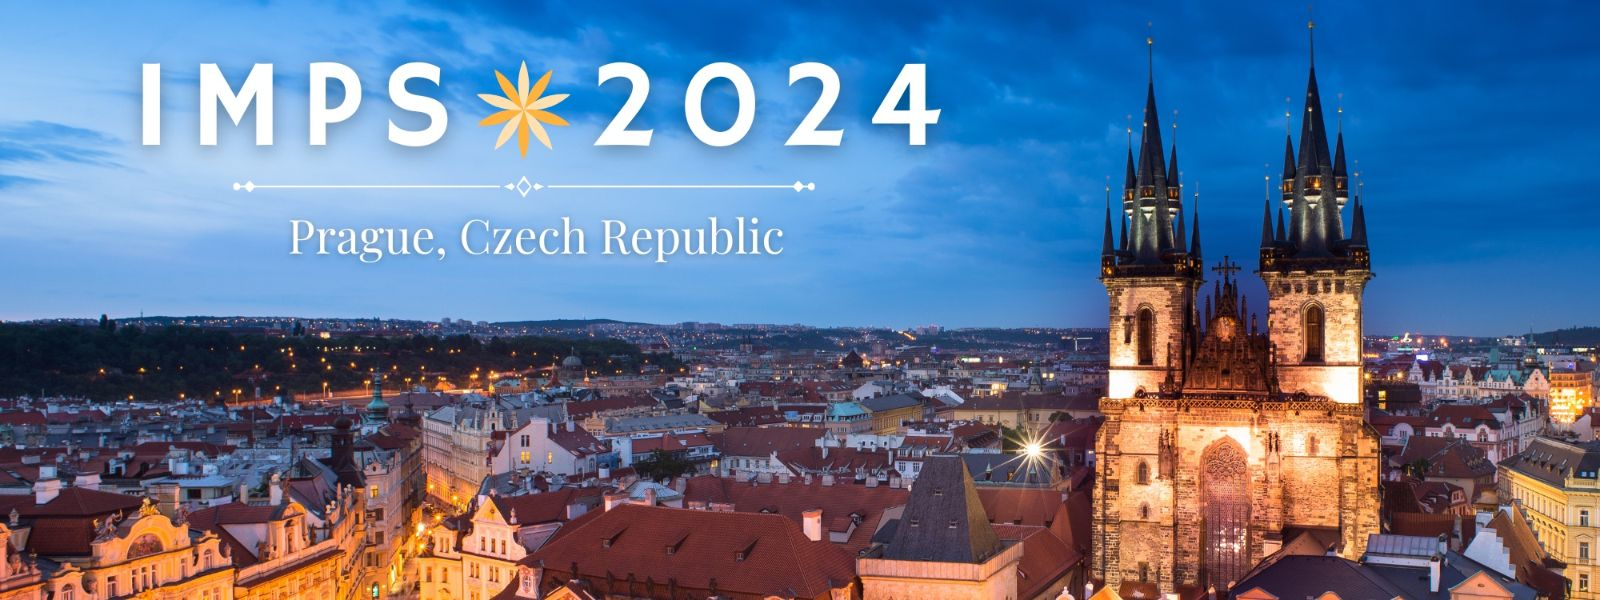
\includegraphics[width=20cm]{Poster TEX/style/IMPS.png}
  
\includegraphics[width=1\linewidth]{Poster TEX/style/qr-code.png}
  
\end{minipage}
\end{figure}

% Header formatting %%%%%%%%%%%%%%%%%%%%%%%%%%%%%%%%%%%%%%%%%%%%%%%%%%%%%%%%%%%%
% The header is divided into two boxes, on the left is the text and on the right is the image
\begin{minipage}[t]{.7\linewidth}
\vfill
\makeatletter
\raggedright{\fontsize{130pt}{100pt}\selectfont\color{uzhblau100}\textbf{{\@title}}\par}
\makeatother
\color{Black}
\vspace{1cm}
\end{minipage}
% Author(s) %%%%%%%%%%%%%%%%%%%%%%%%%%%%%%%%%%%%%%%%%%%%%%%%%%%%%%%%%%%%%%%%%%%%
\begin{minipage}[t]{.3\linewidth}
\vfill
\raggedleft
\large
\textbf{Jiří Novák}\textsuperscript{1,2,3} 
\textbf{Carolin Strobl}\textsuperscript{1,2}
\textbf{Matthias Templ}\textsuperscript{2,3} \\
\vspace{0.2cm}
\large
\textsuperscript{1} University of Zürich \\
\textsuperscript{2} University of Applied Sciences and Arts Northwestern Switzerland  \\
\textsuperscript{3} Swiss Data Anonymization Competence Center
%\texttt{you@uzh.ch}%\\ % add your email
\end{minipage}

\vspace{1cm}

%%%%%%%%%%%%%%%%%%%%%%%%%%%%%%%%%%%%%%%%%%%%%%%%%%%%%%%%%%%%%%%%%%%%%%%%%%%%%%%%
%%%%%%%%%%%%%%%%%%%%%%%%%%%%%%%%%%%%%%%%%%%%%%%%%%%%%%%%%%%%%%%%%%%%%%%%%%%%%%%%
% POSTER BODY %%%%%%%%%%%%%%%%%%%%%%%%%%%%%%%%%%%%%%%%%%%%%%%%%%%%%%%%%%%%%%%%%%
\begin{multicols}{3} % This is how many columns your poster will be broken into

%\large %font size
\normalsize
%%%%%%%%%%%%%%%%%%%%%%%%%%%%%%%%%%%%%%%%%%%%%%%%%%%%%%%%%%%%%%%%%%%%%%%%%%%%%%%%
% Background %%%%%%%%%%%%%%%%%%%%%%%%%%%%%%%%%%%%%%%%%%%%%%%%%%%%%%%%%%%%%%%%%%%
\section{Background}

There is a growing demand for more research data to be made openly available.
The reproducibility of findings is in crisis, and more openly available data would make research more transparent and accessible.

However, \textbf{psychological datasets often include sensitive %demographic and health
personal information that necessitates privacy protection}.
% Many psychological datasets contain \textbf{demographic and health variables} that \textbf{require proper protection against disclosure}.
% Unfortunately, many datasets cannot be publicly available for privacy reasons.

% OPEN SCIENCE, OPEN ACCESS, OPEN DATA %%%%%%%%%%%%%%%%%%%%%%%%%%%%%%%%%%%%%%%%%
\subsection{OPEN SCIENCE, OPEN ACCESS, OPEN DATA}


\includegraphics[width=5cm]{Poster TEX/style/Open Science.png} 
\hspace{\fill} 

\includegraphics[width=10cm]{Poster TEX/style/Open access (4).png}
\hspace{\fill} 

\includegraphics[width=5cm]{Poster TEX/style/Open data.png}

%Research d
Data that results from publicly funded research should be:

%\color{uzhockerrot100}
\begin{itemize}
\item \textbf{Findable, Accessible, Interoperable, Reusable} (‘\textbf{FAIR} principles’) \cite{2022_EUA} \cite{EU_2018-790}
%\color{black}
 therefore replicable, transparent, shareable, trustworthy, verifiable and accountable.
%\color{uzhockerrot100}
\item \textbf{As open as possible, as closed as necessary.}
\end{itemize}
\color{black}

%\href{https://eur-lex.europa.eu/legal-content/EN/TXT/?uri=CELEX%3A32018H0790&qid=1701691098601}{\color{blue}\underline{Commission Recommendation (EU) 2018/790}} \\
%\href{https://eur-lex.europa.eu/legal-content/EN/TXT/?uri=CELEX%3A32018H0790&qid=1701691098601}{\color{blue}\underline{on access to and preservation of scientific}} \\
%\href{https://eur-lex.europa.eu/legal-content/EN/TXT/?uri=CELEX%3A32018H0790&qid=1701691098601}{\color{blue}\underline{information}}

%%%%%%%%%%%%%%%%%%%%%%%%%%%%%%%%%%%%%%%%%%%%%%%%%%%%%%%%%%%%%%%%%%%%%%%%%%%%%%%%
% Methodology %%%%%%%%%%%%%%%%%%%%%%%%%%%%%%%%%%%%%%%%%%%%%%%%%%%%%%%%%%%%%%%%%%
\section{Methodology}

% A key concern with the disclosure of personal data is whether an attacker can gain any new information about an individual. 
% An attacker can gain new information about an individual. 
% JN: It sounds so hollow just like this.

% To enable dissemination and, therefore, to open data, researchers may use methods of \textbf{Statistical Disclosure Control (SDC)} \cite{2017_Templ}. %\cite{2012_Hundepool}.

Released data can provide attackers with new information about specific respondents. For safe dissemination, researchers may use \textbf{Statistical Disclosure Control} (SDC) methods \cite{2017_Templ}:

%\vspace{1cm}
\begin{itemize}
    \item[\ding{228}] The traditional approach to protect data
        \begin{itemize}
            \item[\textbullet] \textbf{Non-perturbation methods} (partially suppressing or reducing details) e.g. Local suppression, %(delete high-risk records)
            Global recoding, %(create broader categories)
            Top and bottom coding, Sampling  
            \item[\textbullet] \textbf{Perturbation methods} (modifying data) \\ %(add noise or alter data so it modifies  data) \
            e.g. Adding noise, Record swapping,  Microaggregation
        \end{itemize}   
\end{itemize}

\begin{itemize}
     \item[\ding{228}] \textbf{Synthetic data generation} to create artificial data that mimics the original data and can be safely disseminated
        \begin{itemize}
            %\item[\textbullet] \textbf{Parametric methods} (statistical models)
            %\item[\textbullet] \textbf{Non-parametric methods} (machine learning, \\ neural networks - GAN)
            \item[\textbullet] \textbf{Joint modeling}  - captures entire data distribution simultaneously, e.g. neural networks (GAN)
            \item[\textbullet] \textbf{Conditional/sequential modeling} - generates data variable by variable, e.g. parametric (regression) or non-parametric (CART) methods
        \end{itemize}        
\end{itemize}

%\columnbreak % Force the end of the column -------------------------------------

%%%%%%%%%%%%%%%%%%%%%%%%%%%%%%%%%%%%%%%%%%%%%%%%%%%%%%%%%%%%%%%%%%%%%%%%%%%%%%%%
% Example of anonymization %%%%%%%%%%%%%%%%%%%%%%%%%%%%%%%%%%%%%%%%%%%%%%%%%%%%%
\section{Example of synthetic data generation}

Let's suppose that we are obliged to share data 
% openly while protecting participants' privacy and aligning with open science goals.
while reducing the risk that an attacker learns something new about respondents.

\begin{itemize}
    \item[\ding{228}] \textbf{Dataset Description}
        \begin{itemize}   
            \item[\textbullet] The data for this example is from the Answers to the Machivallianism Test, a version of the MACH-IV from Christie and Geis (1970) \cite{Data}.
            \item[\textbullet] Includes variables about Likert-rated items and demographic/other items.
        \end{itemize}
%The dataset utilized for this anonymization example is sourced from the Alzheimer's Disease Dataset \cite{2024_Alzheimer}. It includes variables such as patient info, demographics, lifestyle, medical history, clinical measurements, symptoms, and diagnosis.
    \item[\ding{228}] \textbf{Anonymization tools}
        \begin{itemize}   
            \item[\textbullet] Synthetization was performed using the R package  \href{https://cran.r-project.org/web/packages/synthpop/index.html} {\color{blue}\underline{synthpop}} \cite{2022_Synthpop} with method CART.
            \item[\textbullet]  For traditional SDC methods we would use package \href{https://cran.r-project.org/web/packages/sdcMicro/index.html}{\color{blue}\underline{sdcMicro}} \cite{2024_Sdcmicro} or for simulation of  complex synthetic data package \href{https://cran.r-project.org/web/packages/simPop/index.html}{\color{blue}\underline{simPop}}~\cite{2022_Simpop}.
        \end{itemize}
%The anonymization with synthetization may be performed in R package \href{https://cran.r-project.org/web/packages/synthpop/index.html}{\color{blue}\underline{synthpop}} \cite{2022_Synthpop}. For SDC methods we would use package \href{https://cran.r-project.org/web/packages/sdcMicro/index.html}{\color{blue}\underline{sdcMicro}} or for complex data package \href{https://cran.r-project.org/web/packages/simPop/index.html}{\color{blue}\underline{simPop}}.
\end{itemize}

 %In our example, we evaluated the utility of synthetic data by comparing original and synthetic datasets on several metrics.

\columnbreak % Force the end of the column -------------------------------------

% Data utility %%%%%%%%%%%%%%%%%%%%%%%%%%%%%%%%%%%%%%%%%%%%%%%%%%%%%%%%%%%%%%%%%
\subsection{Data utility}

\textit{Data utility} refers to the \textbf{usefulness of the data for the intended purpose}. 
The utility of synthetic data is measured by how the results from analyses of synthetic data differ from those derived from the real data.
There is also a \textbf{risk-utility trade-off}.
% Balancing data utility and privacy is essential. High utility ensures synthetic data's effectiveness for research, while privacy measures minimize re-identification risk.

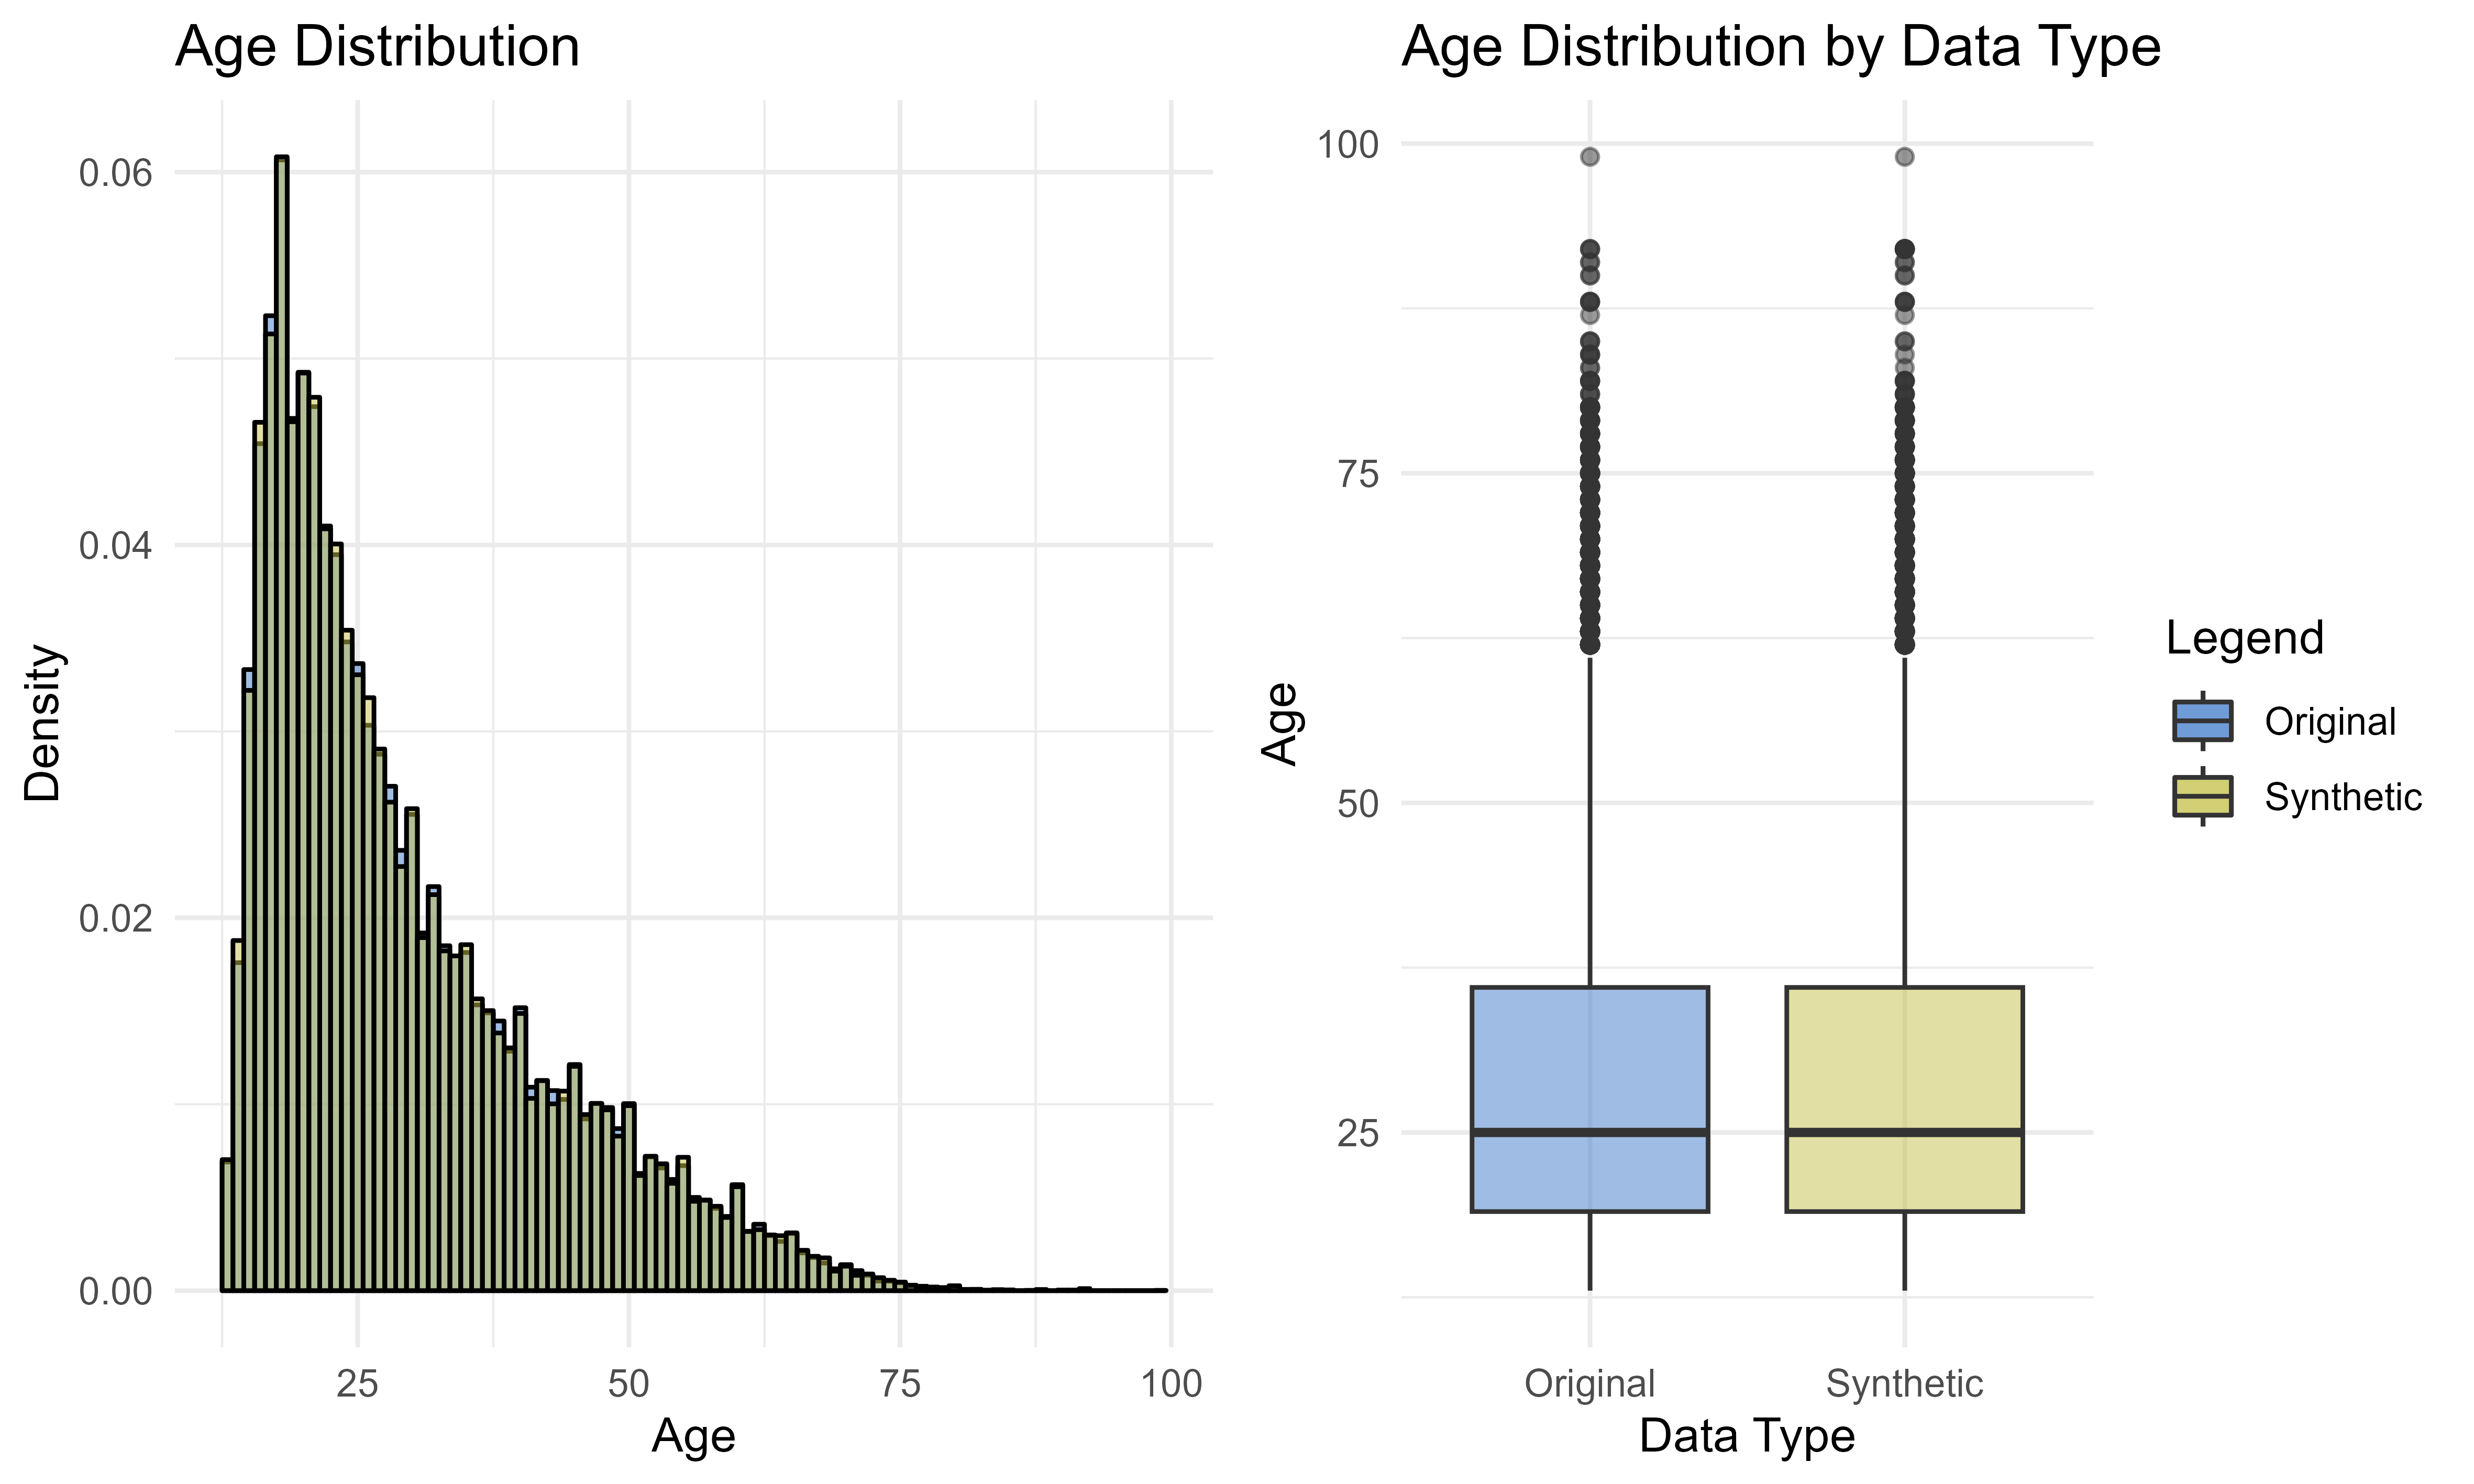
\includegraphics[width=1\linewidth]{Poster TEX/figures/Hist_box_age_v5.png}
\captionof{figure}{Difference in age distribution between Original and Synthetic dataset}

\vspace{1cm}

The plot for the variable shows the age distribution for both the original and synthetic datasets.
The similarity in the histograms and boxplots suggests that the synthetic data maintains the original data's variability and distribution characteristics.

\vspace{1cm}

Propensity Mean Squared Error ($pMSE$) and its Standardized Ratio ($S_{pMSE}$) are used to compare the similarity between synthetic and original datasets. $pMSE$ is derived from a propensity score model, where the propensity score is the probability that a given data point belongs to the synthetic dataset rather than the original dataset. A lower $pMSE$ indicates better similarity between the datasets.
$S_{pMSE}$ accounts for the expected mean squared error if the datasets were perfectly separable. It normalizes the $pMSE$ by dividing it by the $pMSE$ of a "null" model where the datasets are completely random.

\begin{equation}
\text{$pMSE$} = \frac{1}{N} \sum_{i=1}^{N} (P_i - Y_i)^2 \quad
S_{pMSE} = \frac{\text{$pMSE$}}{\text{$pMSE$}_{\text{null}}}
\end{equation}

\vspace{1cm}

\begin{center}
\begin{tabular}{lrrr}
  \toprule
Variable & $pMSE$ & $S_{pMSE}$ & df \\ 
  \midrule
  age & 0.000001 & 0.380055 & 4 \\ 
  gender & 0.000000 & 0.456684 & 1 \\ 
  married & 0.000001 & 0.296588 & 3 \\ 
  religion & 0.000010 & 0.927885 & 12 \\ 
  education & 0.000002 & 0.684630 & 3 \\ 
  urban & 0.000001 & 0.458887 & 3 \\ 
  engnat & 0.000002 & 1.952587 & 1 \\ 
  hand & 0.000001 & 0.220005 & 3 \\ 
  orientation & 0.000002 & 0.366338 & 5 \\ 
%  race & 0.000008 & 1.262795 & 7 \\ 
%  voted & 0.000001 & 0.435028 & 2 \\ 
%  familysize & 0.000006 & 3.208686 & 2 \\ 
   \bottomrule
\end{tabular}
\caption{Comparison of $pMSE$ and $S_{pMSE}$  for different variables} 
\label{tab:pmse}
\end{center}

The variable \textit{age} shows a $pMSE$ of 0.000001 and an $S_{pMSE}$ of 0.380055, indicating a close match between the synthetic and original datasets. Similarly, \textit{gender} exhibits an extremely low $pMSE$ and an $S_{pMSE}$ of 0.456684, suggesting excellent similarity. For \textit{married} status, the $pMSE$ is 0.000001 with an $S_{pMSE}$ of 0.296588, reflecting strong similarity between the datasets.

The variable \textit{religion} has a slightly higher $pMSE$ of 0.000010 and an $S_{pMSE}$ of 0.927885, indicating that while the datasets are fairly similar, some differences exist. \textit{Education} shows moderate similarity with a $pMSE$ of 0.000002 and an $S_{pMSE}$ of 0.684630. The \textit{urban} variable has a low $pMSE$ of 0.000001 and an $S_{pMSE}$ of 0.458887, denoting good similarity.

However, \textit{engnat} (native English speaker status) presents a higher $S_{pMSE}$ of 1.952587, indicating differences between the datasets. Variable \textit{hand} demonstrates excellent similarity with a $pMSE$ of 0.000001 and an $S_{pMSE}$ of 0.220005. \textit{Orientation} is similar, with a $pMSE$ of 0.000002 and an $S_{pMSE}$ of 0.366338.

%Race has a $pMSE$ of 0.000008 and an $S_{pMSE}$ of 1.262795, suggesting some distinguishable differences between the datasets. The variable voted shows strong similarity with a $pMSE$ of 0.000001 and an $S_{pMSE}$ of 0.435028. Lastly, familysize stands out with the highest $S_{pMSE}$ of 3.208686 and a $pMSE$ of 0.000006, indicating significant differences between the original and synthetic data for this variable. Overall, while most variables show strong similarity between the datasets, engnat, race, and familysize may require further refinement in the synthetic data generation process to achieve better alignment with the original data.


\columnbreak % Force the end of the column -------------------------------------

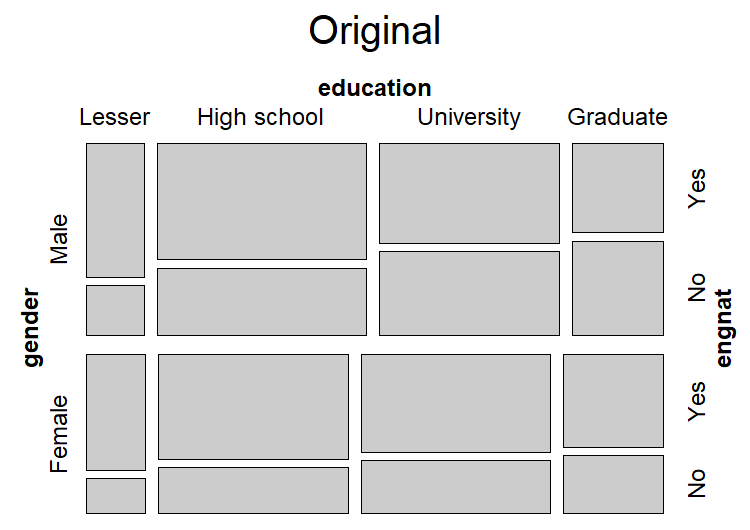
\includegraphics[width=1\linewidth]{Poster TEX/figures/Mosaic_orig_v5.png}

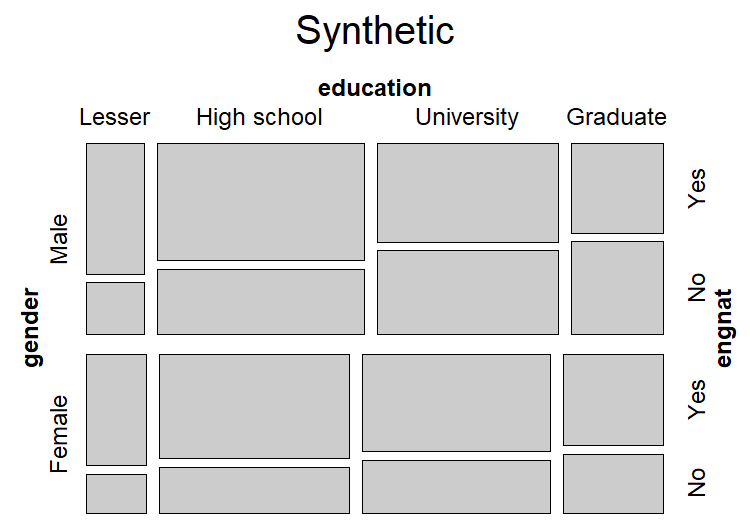
\includegraphics[width=1\linewidth]{Poster TEX/figures/Mosaic_synt_v5.png}
\captionof{figure}{Mosaic plots for selected variables}

\vspace{1cm}

The mosaic plots display differences in structure for categorical data. In this case, the synthetic and original datasets show highly similar distributions across the variables \textit{gender}, \textit{education}, and \textit{engnat}. This similarity indicates that the synthetic data effectively preserves the relationships and proportions present in the original data and its analytical utility.

%%%%%%%%%%%%%%%%%%%%%%%%%%%%%%%%%%%%%%%%%%%%%%%%%%%%%%%%%%%%%%%%%%%%%%%%%%%%%%%%
% FORTHCOMING RESEARCH %%%%%%%%%%%%%%%%%%%%%%%%%%%%%%%%%%%%%%%%%%%%%%%%%%%%%%%%%
\section{Forthcoming Research}

The goal of our SNSF\textsuperscript{\ding{107}}-funded project is developing and implementing innovative tools for generating synthetic longitudinal data with a focus on disclosure risk.

%In an SNSF\textsuperscript{\ding{107}}-funded project, we will focus on anonymizing longitudinal health data and addressing re-identification risk. Our goal is to develop and implement innovative tools for generating synthetic longitudinal data.


%In a project funded by the SNSF~\textsuperscript{\ding{107}}
%\nameref{Acknowledgments}
%we will focus on anonymizing the longitudinal data, including re-identification risk.
%We will focus on the anonymization of longitudinal data.
%The challenges of anonymizing longitudinal data are data granularity, temporal uniqueness, and dynamic features. 
%Given the sensitive nature of health data, we aim to develop and implement innovative tools for generating synthetic longitudinal data.

%%%%%%%%%%%%%%%%%%%%%%%%%%%%%%%%%%%%%%%%%%%%%%%%%%%%%%%%%%%%%%%%%%%%%%%%%%%%%%%%
% REFERENCES %%%%%%%%%%%%%%%%%%%%%%%%%%%%%%%%%%%%%%%%%%%%%%%%%%%%%%%%%%%%%%%%%%%
\singlespacing
\small
%\nocite{*} % Print all references regardless of whether they were cited in the poster or not
%\bibliographystyle{plain} % Plain referencing style
%\bibliographystyle{plainurl}
%\bibliographystyle{ieeetr}
\bibliographystyle{unsrt}
\bibliography{bib} % Use the example bibliography file sample.bib

%%%%%%%%%%%%%%%%%%%%%%%%%%%%%%%%%%%%%%%%%%%%%%%%%%%%%%%%%%%%%%%%%%%%%%%%%%%%%%%%
% Acknowledgments %%%%%%%%%%%%%%%%%%%%%%%%%%%%%%%%%%%%%%%%%%%%%%%%%%%%%%%%%%%%%%
\subsection{\textsuperscript{\ding{107}}Acknowledgments}
\label{Acknowledgments}

\normalsize
This work was funded by the Swiss National Science Foundation (SNSF) with grant number 211751: "\textit{Harnessing event and longitudinal data in industry and health sector through privacy preserving technologies}".


%%%%%%%%%%%%%%%%%%%%%%%%%%%%%%%%%%%%%%%%%%%%%%%%%%%%%%%%%%%%%%%%%%%%%%%%%%%%%%%%
% QR code %%%%%%%%%%%%%%%%%%%%%%%%%%%%%%%%%%%%%%%%%%%%%%%%%%%%%%%%%%%%%%%%%%%%%%
% 
\includegraphics[width=1\linewidth]{Poster TEX/style/qr-code.png}

%%%%%%%%%%%%%%%%%%%%%%%%%%%%%%%%%%%%%%%%%%%%%%%%%%%%%%%%%%%%%%%%%%%%%%%%%%%%%%%%
%\columnbreak % Force the end of the column 
%%%%%%%%%%%%%%%%%%%%%%%%%%%%%%%%%%%%%%%%%%%%%%%%%%%%%%%%%%%%%%%%%%%%%%%%%%%%%%%%
% ILLUSTRATIVE EXAMPLE %%%%%%%%%%%%%%%%%%%%%%%%%%%%%%%%%%%%%%%%%%%%%%%%%%%%%%%%%
%\section{ILLUSTRATIVE EXAMPLE}

% DATA UTILITY %%%%%%%%%%%%%%%%%%%%%%%%%%%%%%%%%%%%%%%%%%%%%%%%%%%%%%%%%%%%%%%%%
%\subsection{DATA UTILITY}

%\vspace{1cm}
%\textbf{Difference in Correlations Between Original and Synthetic dataset}
%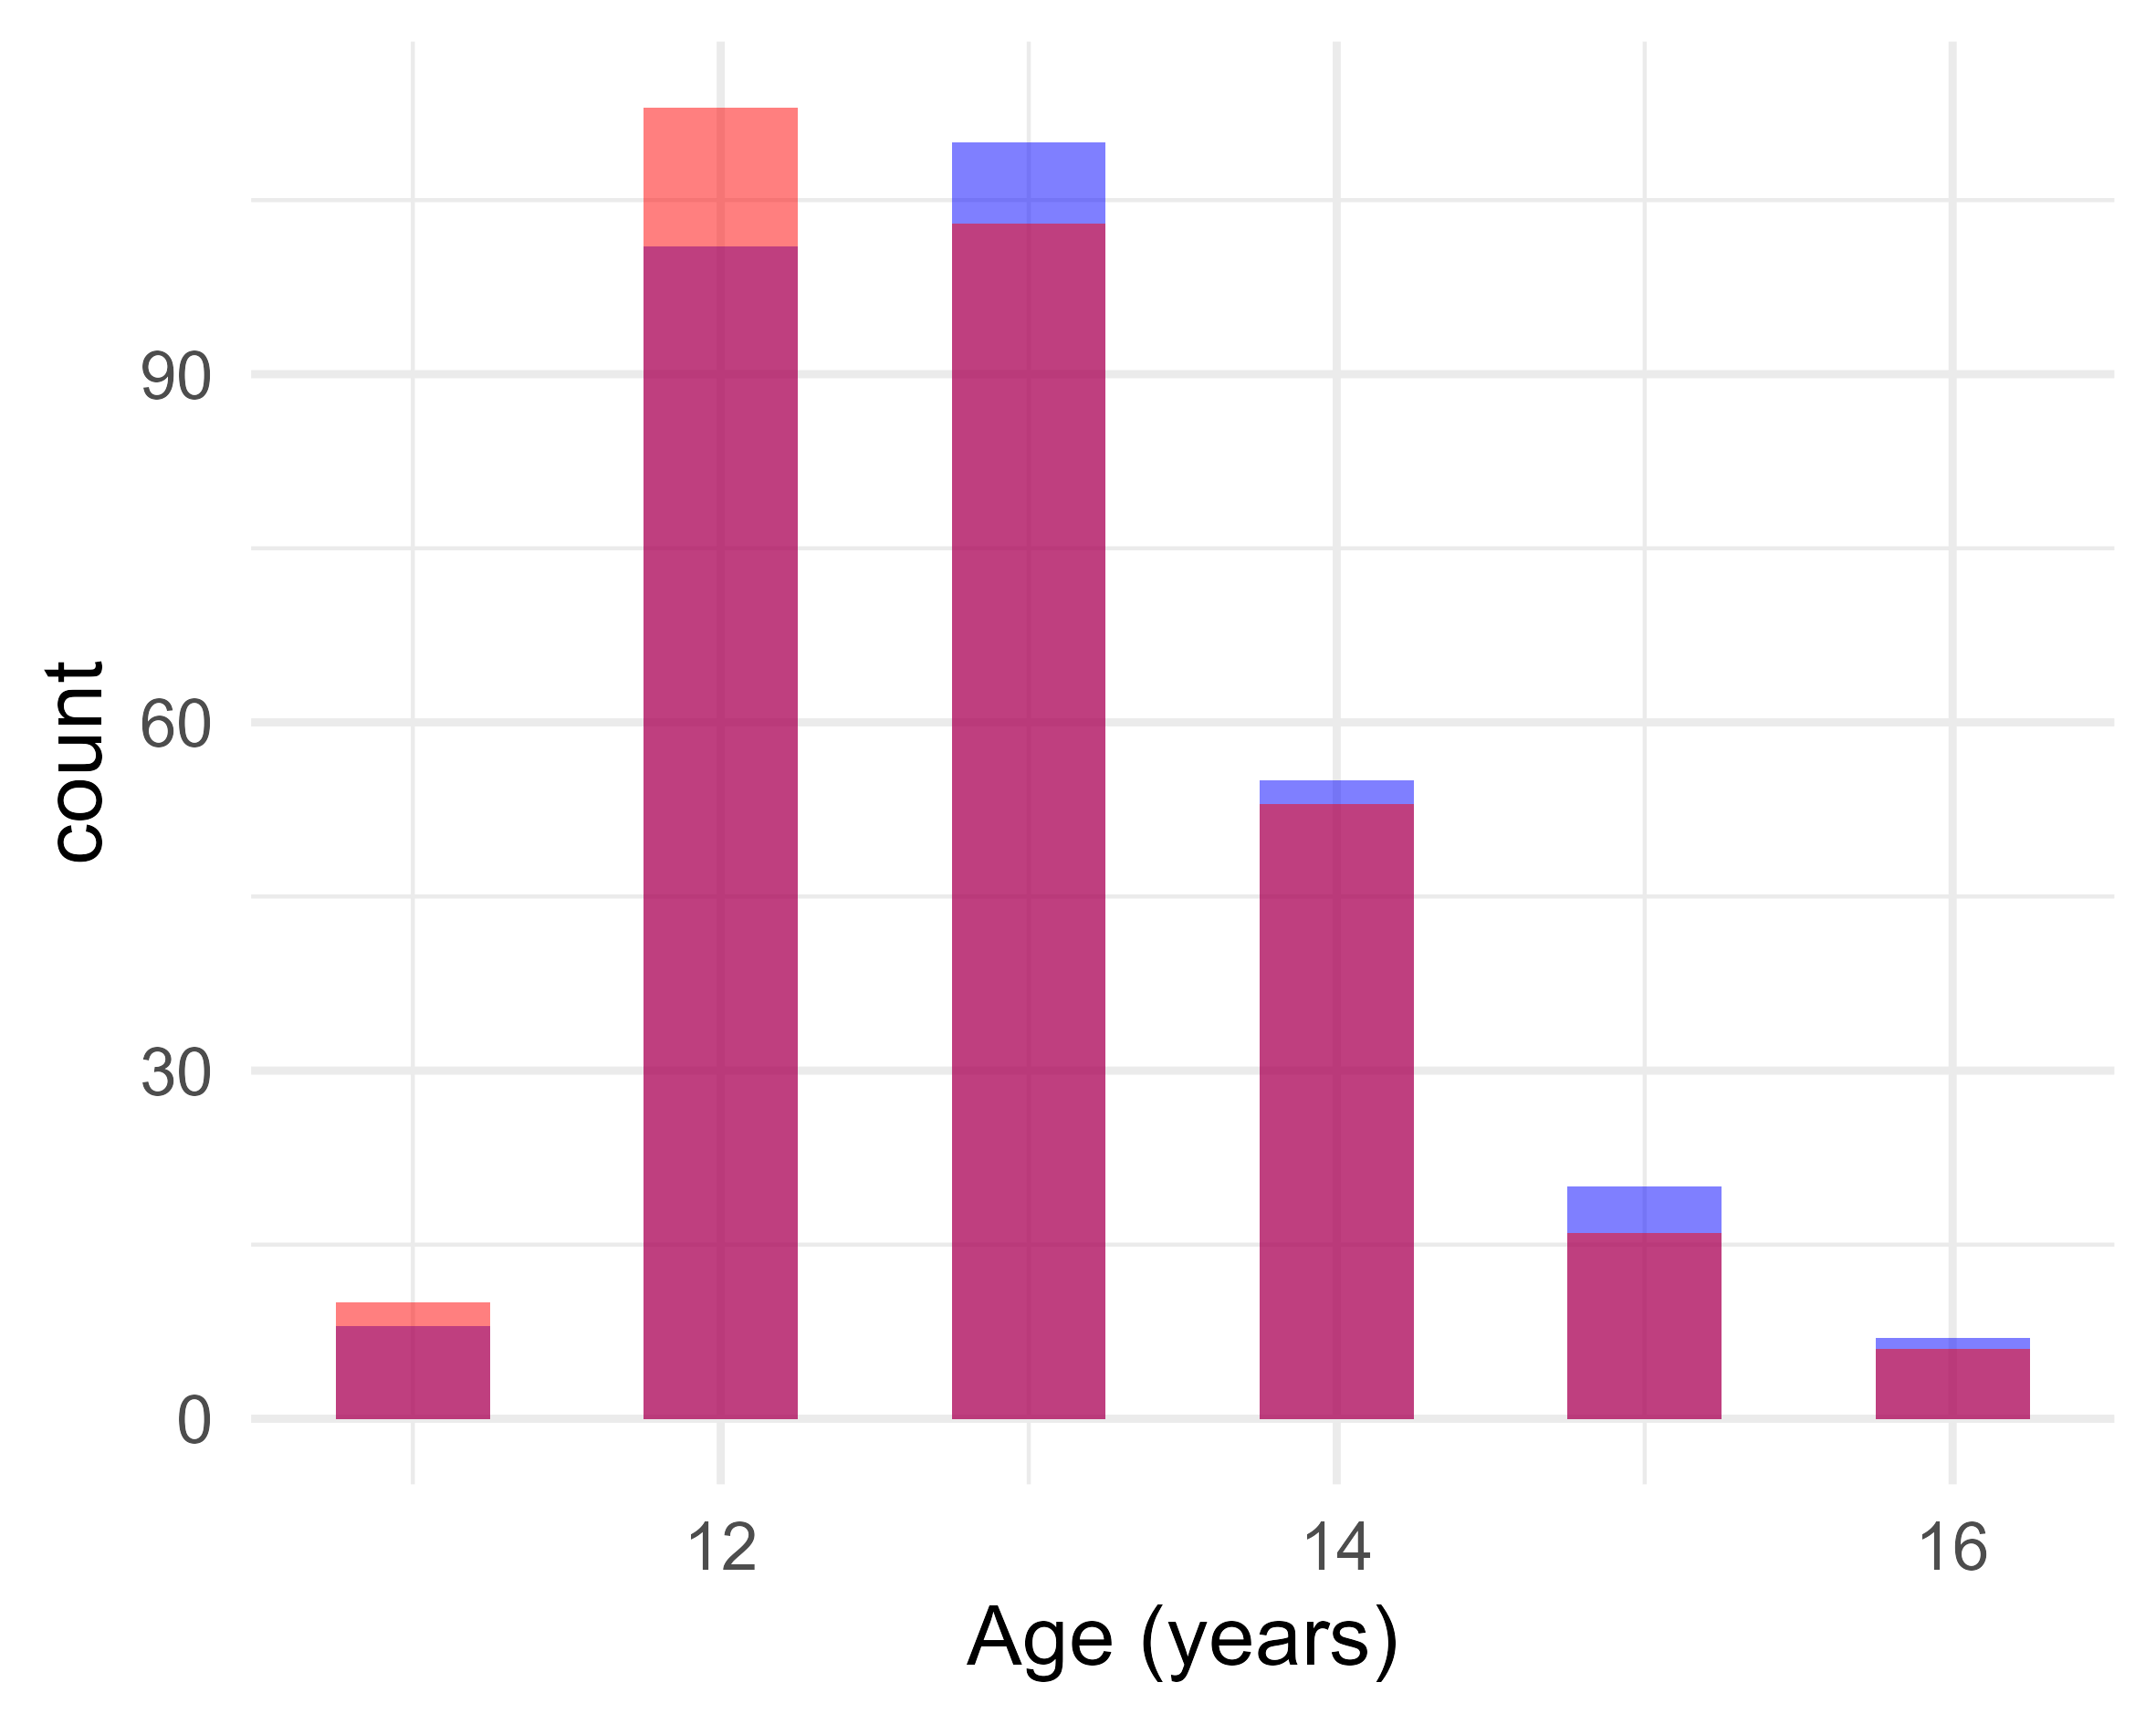
\includegraphics[width=1\linewidth]{Poster TEX/figures/Histogram_ageyr.png}
%\captionof{figure}{Difference in Correlations Between Original and Synthetic dataset}

%\vspace{1cm}
%\textbf{Difference in Correlations Between Original and Synthetic dataset}
%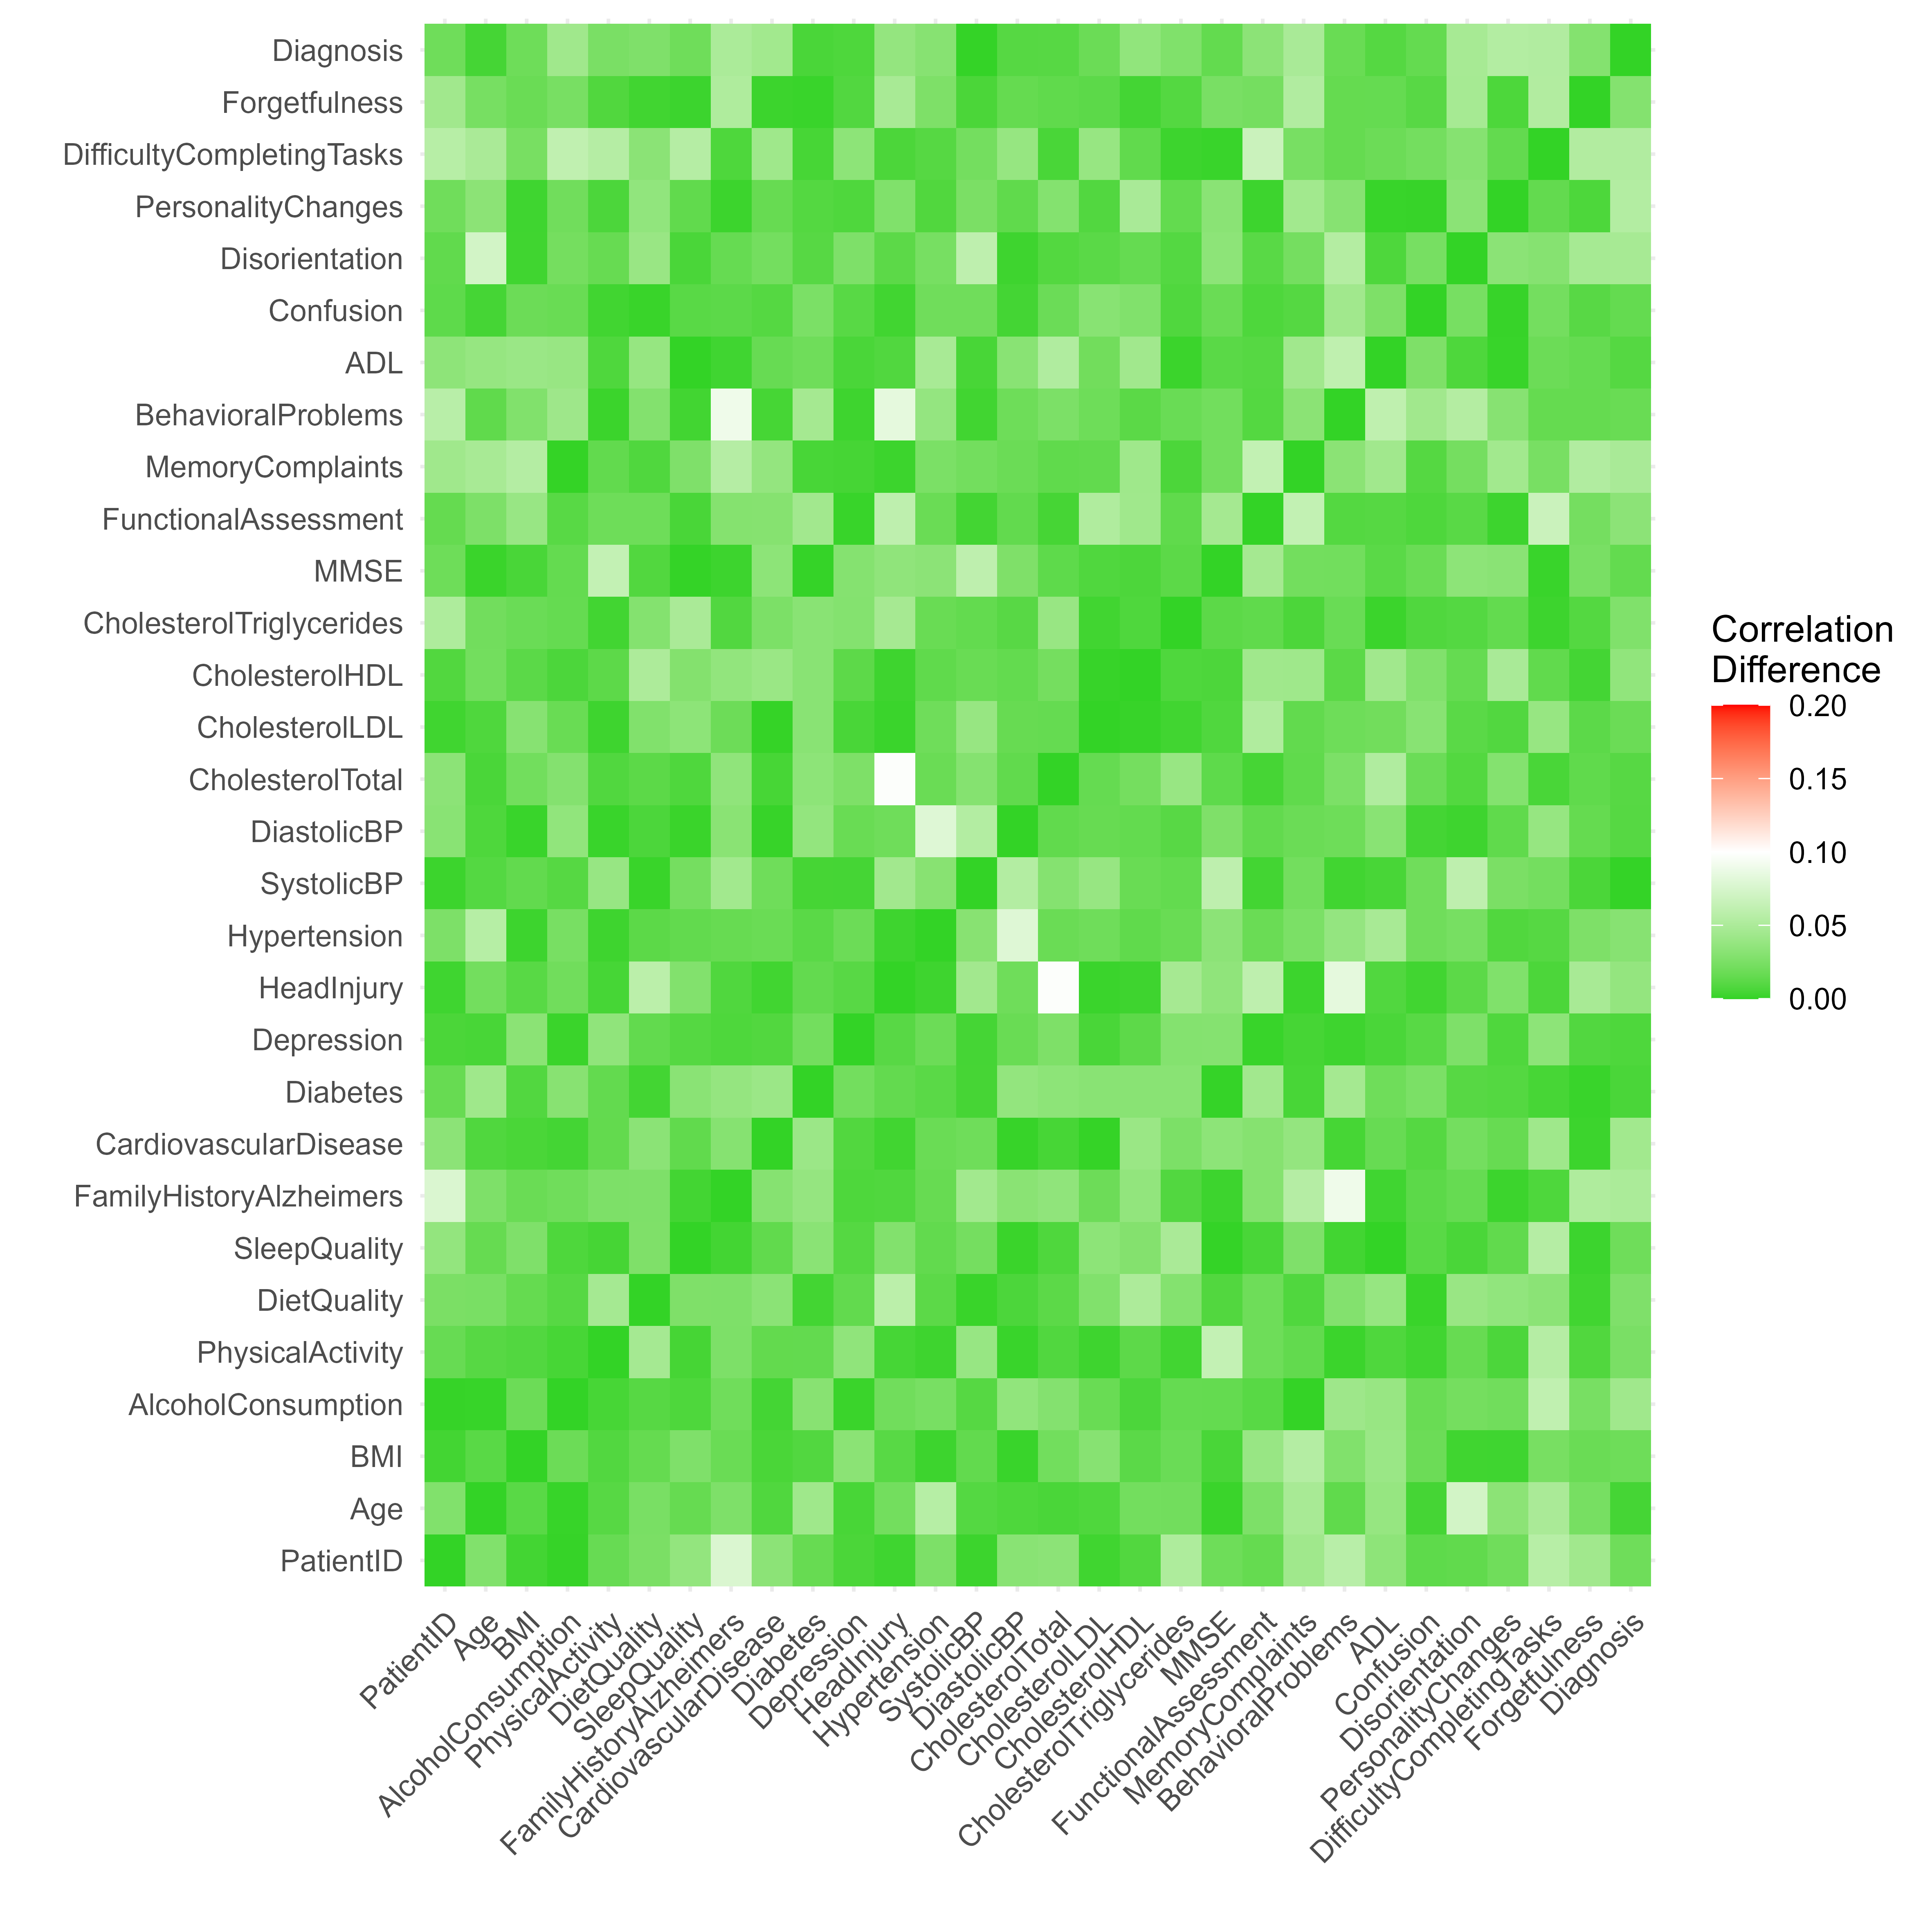
\includegraphics[width=1\linewidth]{Poster TEX/figures/Correlation_Difference.png}
%\captionof{figure}{Difference in correlations between Original and Synthetic dataset}

% \columnbreak % Force the end of the column 

%\vspace{1cm}
%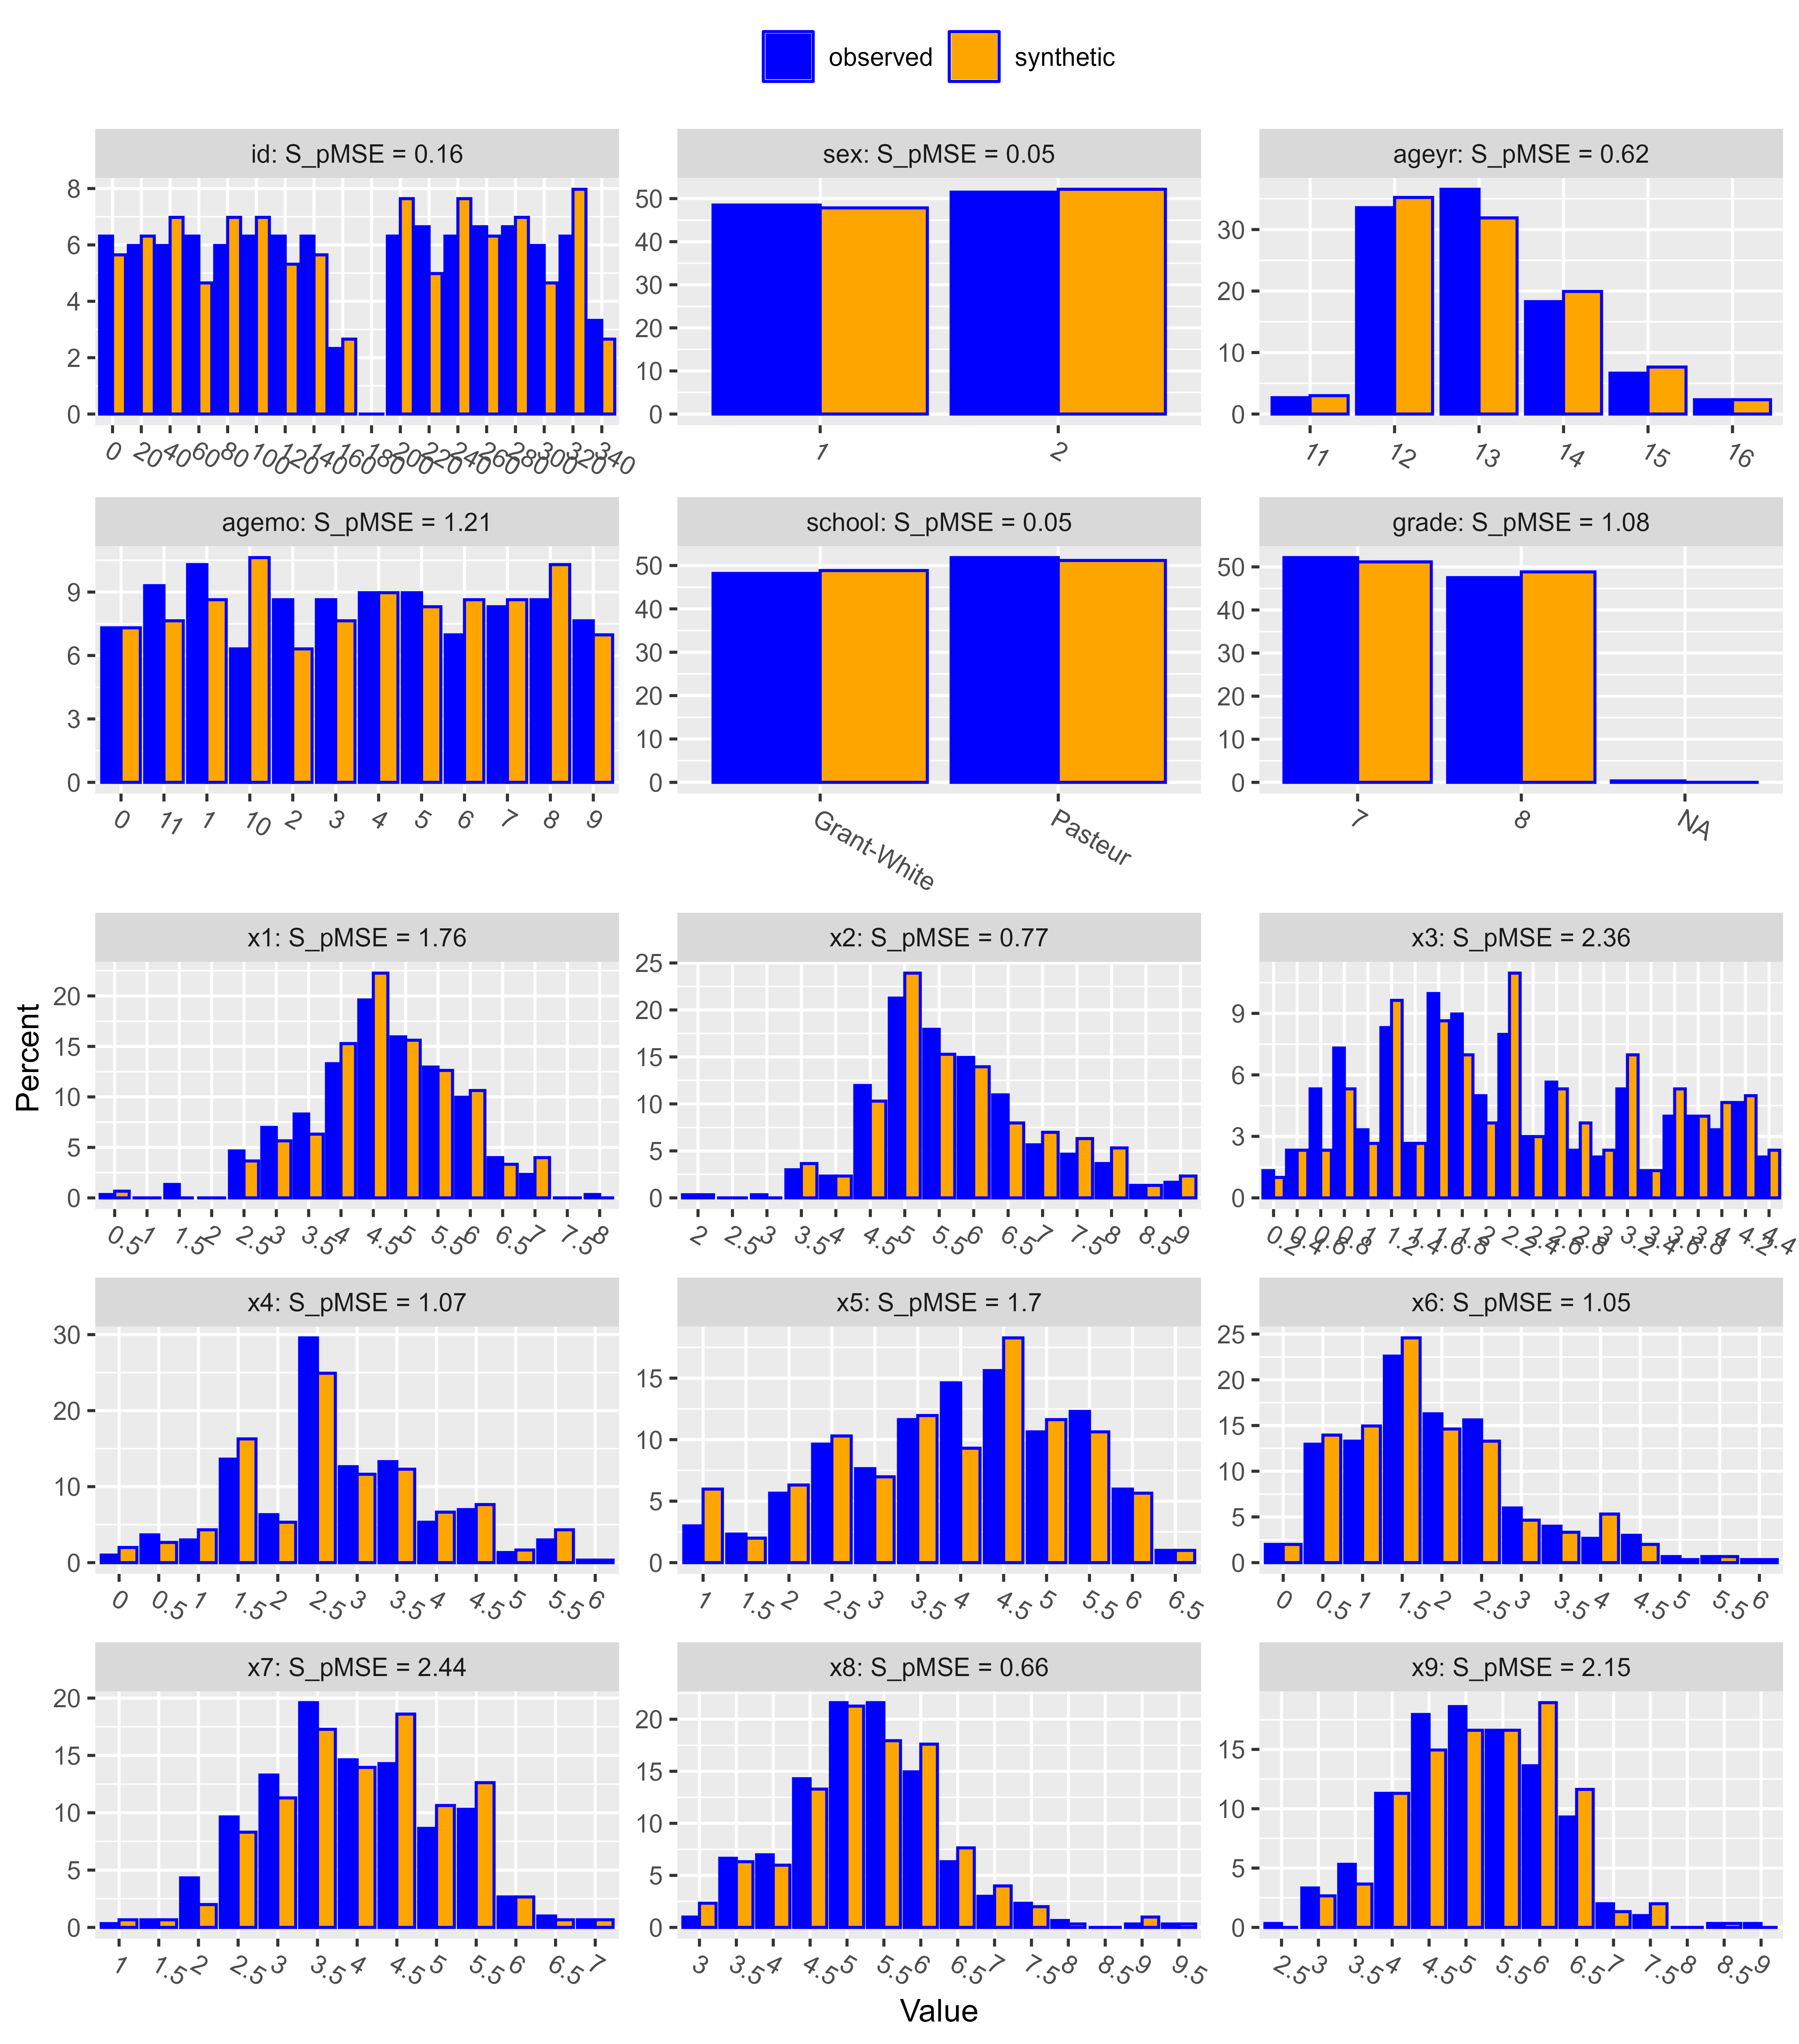
\includegraphics[width=1\linewidth]{Poster TEX/figures/synthpop_compare.png}
%\captionof{figure}{Difference in distributions between Original and Synthetic dataset}

%\vspace{1cm}
% To evaluate the success of the synthetic data generation, we compared the synthetic dataset to the original using visual and statistical methods, focusing on distributions and correlations to ensure accurate representation.
%One approach to assessing the effectiveness of synthetic data generation is to compare the synthetic dataset to the original using both visual and statistical methods, focusing on distributions and correlations to ensure accurate representation.

 
%%%%%%%%%%%%%%%%%%%%%%%%%%%%%%%%%%%%%%%%%%%%%%%%%%%%%%%%%%%%%%%%%%%%%%%%%%%%%%%%
\end{multicols}
\end{document}
%%%%%%%%%%%%%%%%%%%%%%%%%%%%%%%%%%%%%%%%%%%%%%%%%%%%%%%%%%%%%%%%%%%%%%%%%%%%%%%%
%%%%%%%%%%%%%%%%%%%%%%%%%%%%%%%%%%%%%%%%%%%%%%%%%%%%%%%%%%%%%%%%%%%%%%%%%%%%%%%%
%%%%%%%%%%%%%%%%%%%%%%%%%%%%%%%%%%%%%%%%%%%%%%%%%%%%%%%%%%%%%%%%%%%%%%%%%%%%%%%%